%\lipsum[1-20]
\section{Deriving Rates}

\begin{align}
\hat{Q}_{jk} &= Q^0_{jk} \\
	&= S_{jk}e^{\beta_0(E_{jk} - E_j)} \\
E_{jk} &= E_j-\frac{1}{\beta_0}\log\left(\hat{Q}_{jk}/S_{jk}\right)
\end{align}
\section{Self-Assembly Statistics}



\begin{figure}[ht]
\label{fig:OctaCCS}
\centering
  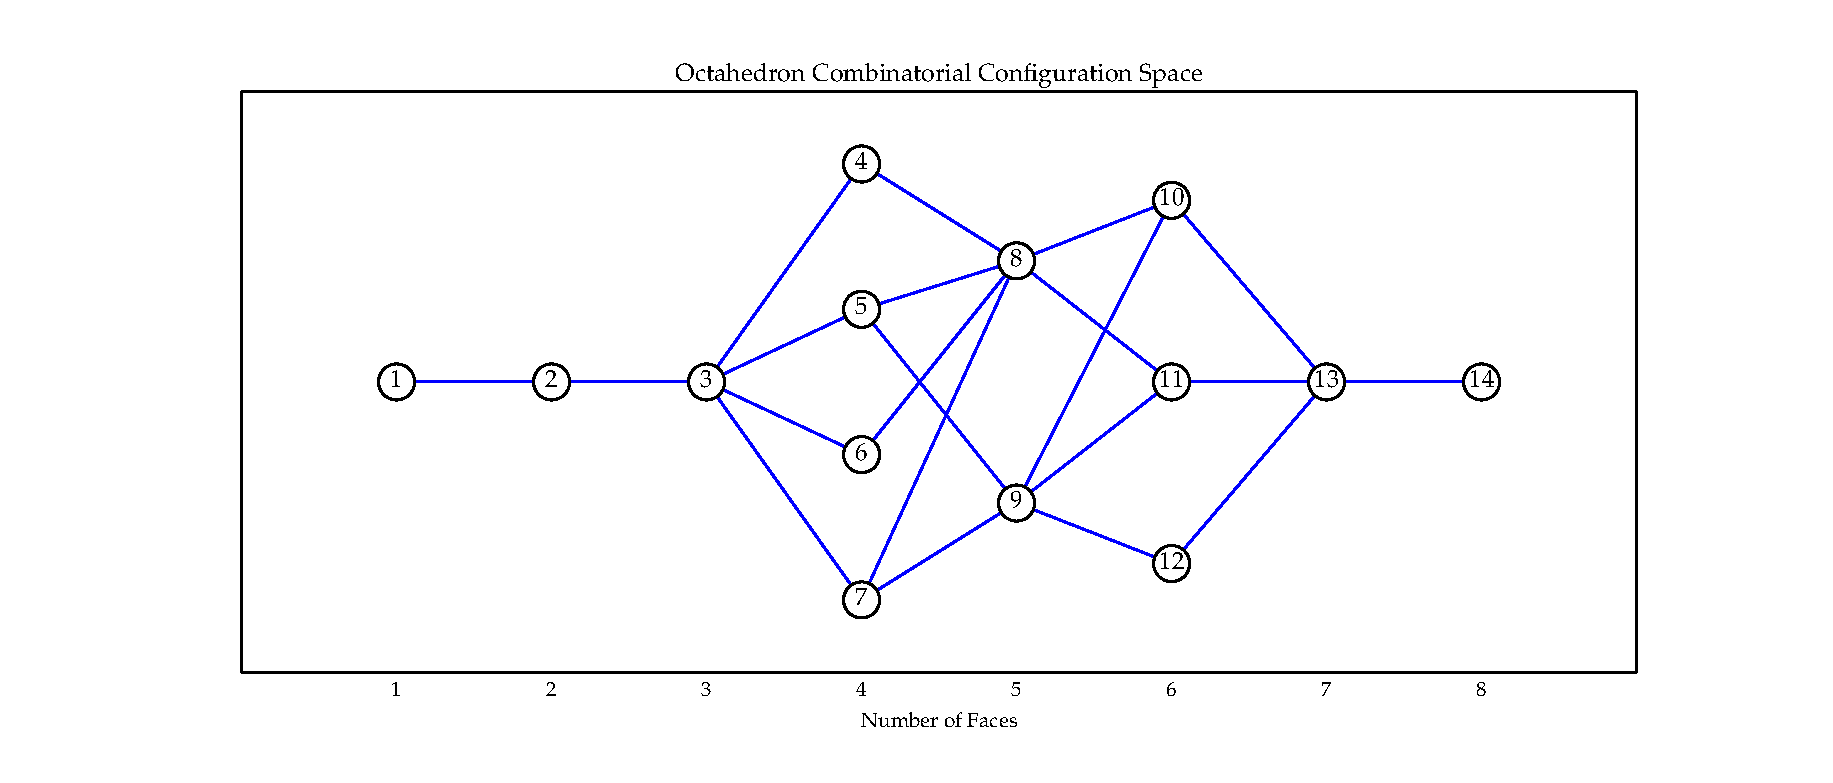
\includegraphics[scale=0.6]{images/octahedron_ccs.eps}
\caption{Combinatorial Configuration space for the Octahedron.}
\end{figure}

\begin{figure}[ht]
\label{fig:OctaPi}
\centering
  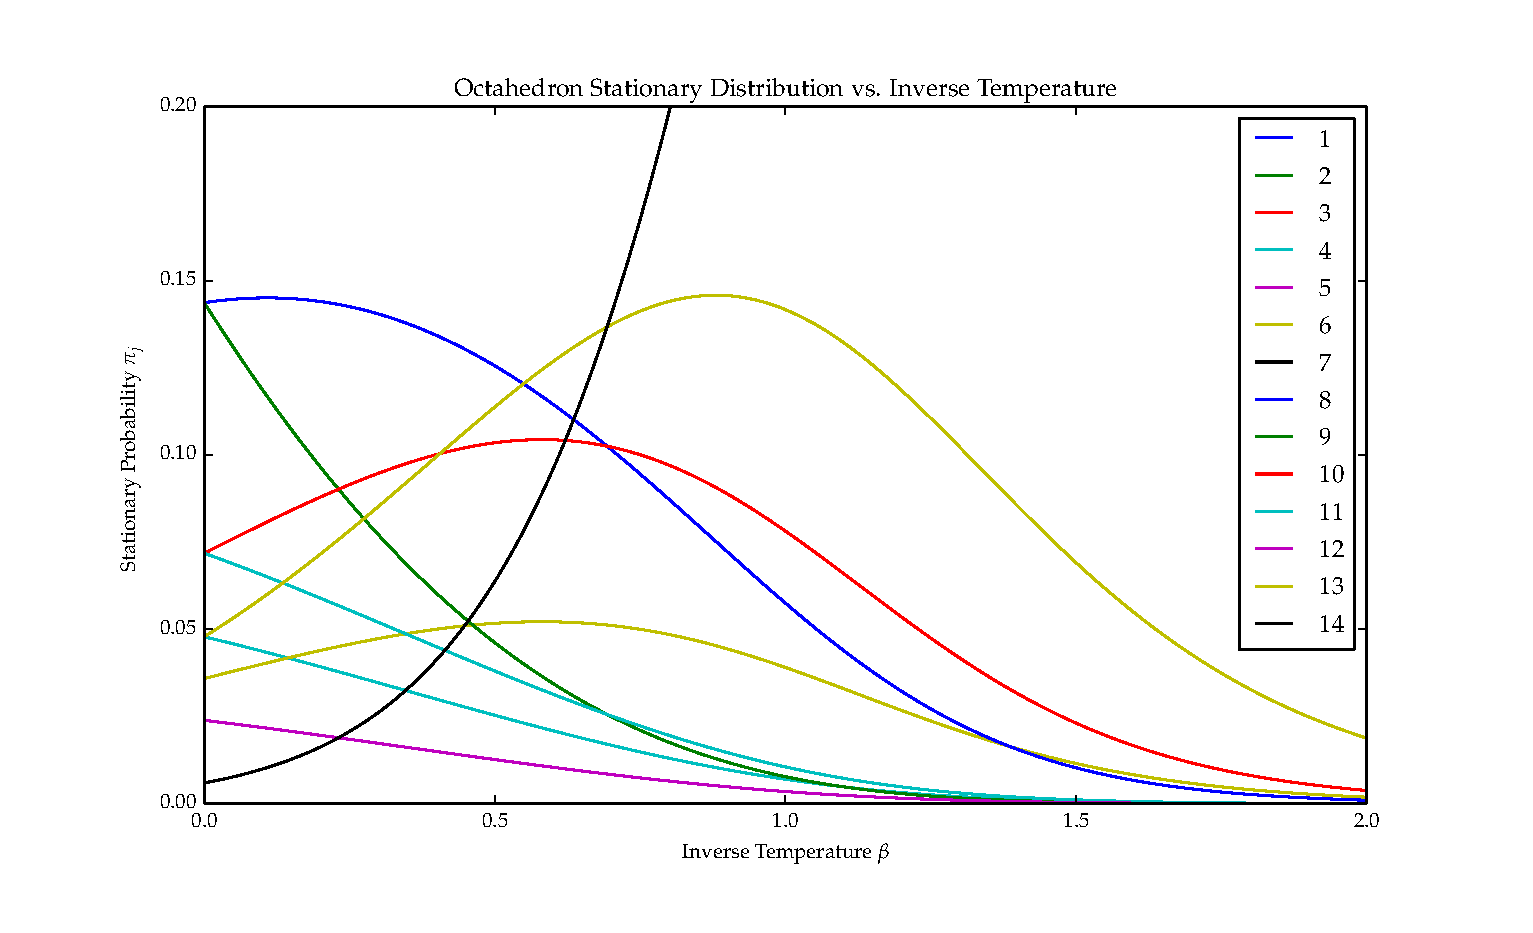
\includegraphics[scale=0.6]{images/octahedron_pi.eps}
\caption{Octahedron stationary distributions as a function of $\beta$.}
\end{figure}

\begin{figure}[ht]
\label{fig:OctaLogPi}
\centering
  \includegraphics[scale=0.6]{images/octahedron_log_pi.eps}
\caption{Natural log of the octahedron stationary distributions as a function of $\beta$.}
\end{figure}

\begin{figure}[ht]
\label{fig:OctaFinDist}
\centering
  \includegraphics[scale=0.6]{images/octahedron_finite_dist.eps}
\caption{Occupation probabilities for Octahedron intermediates as a function of time.}
\end{figure}

\begin{figure}[ht]
\label{fig:OctaPiGrid}
\centering
  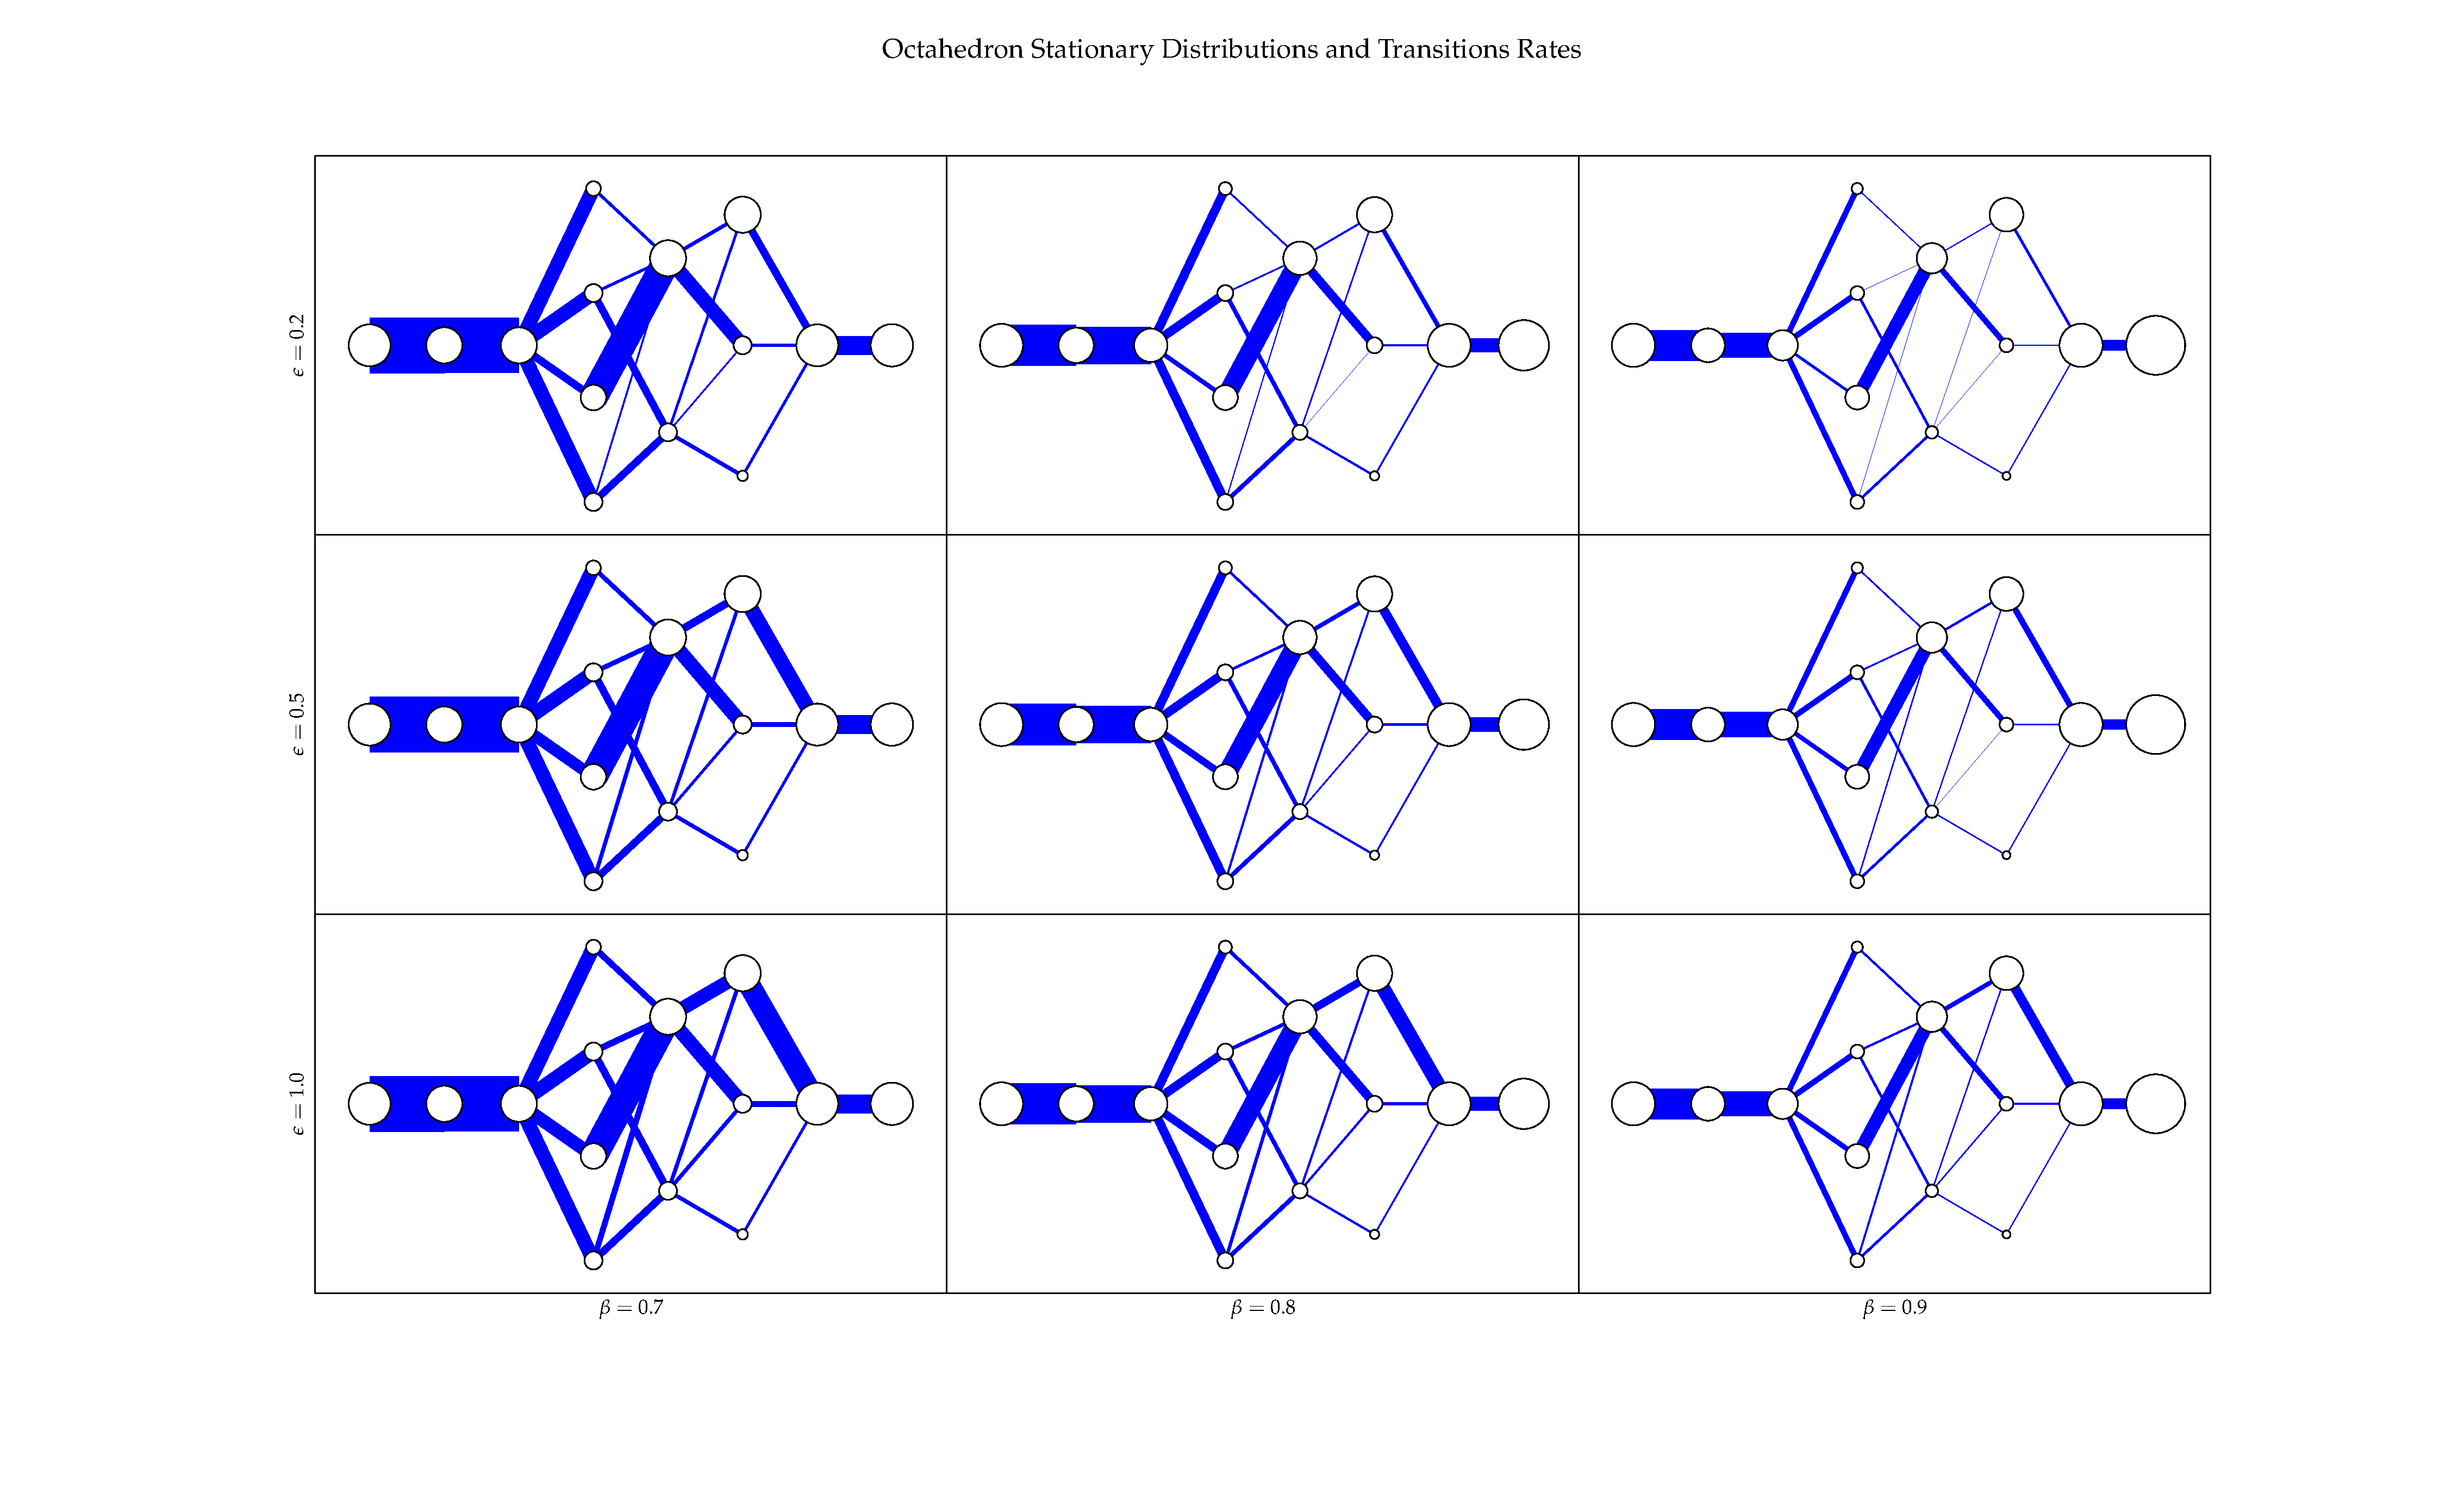
\includegraphics[scale=0.22]{images/octahedron_pi_Q_grid.eps}
\caption{The Affect of $\beta$ and $\epsilon$ on the transitions rates and stationary distribution of the Octahedron combinatorial configuration space.}
\end{figure}

\begin{figure}[ht]
\label{fig:OctaTau}
\centering
  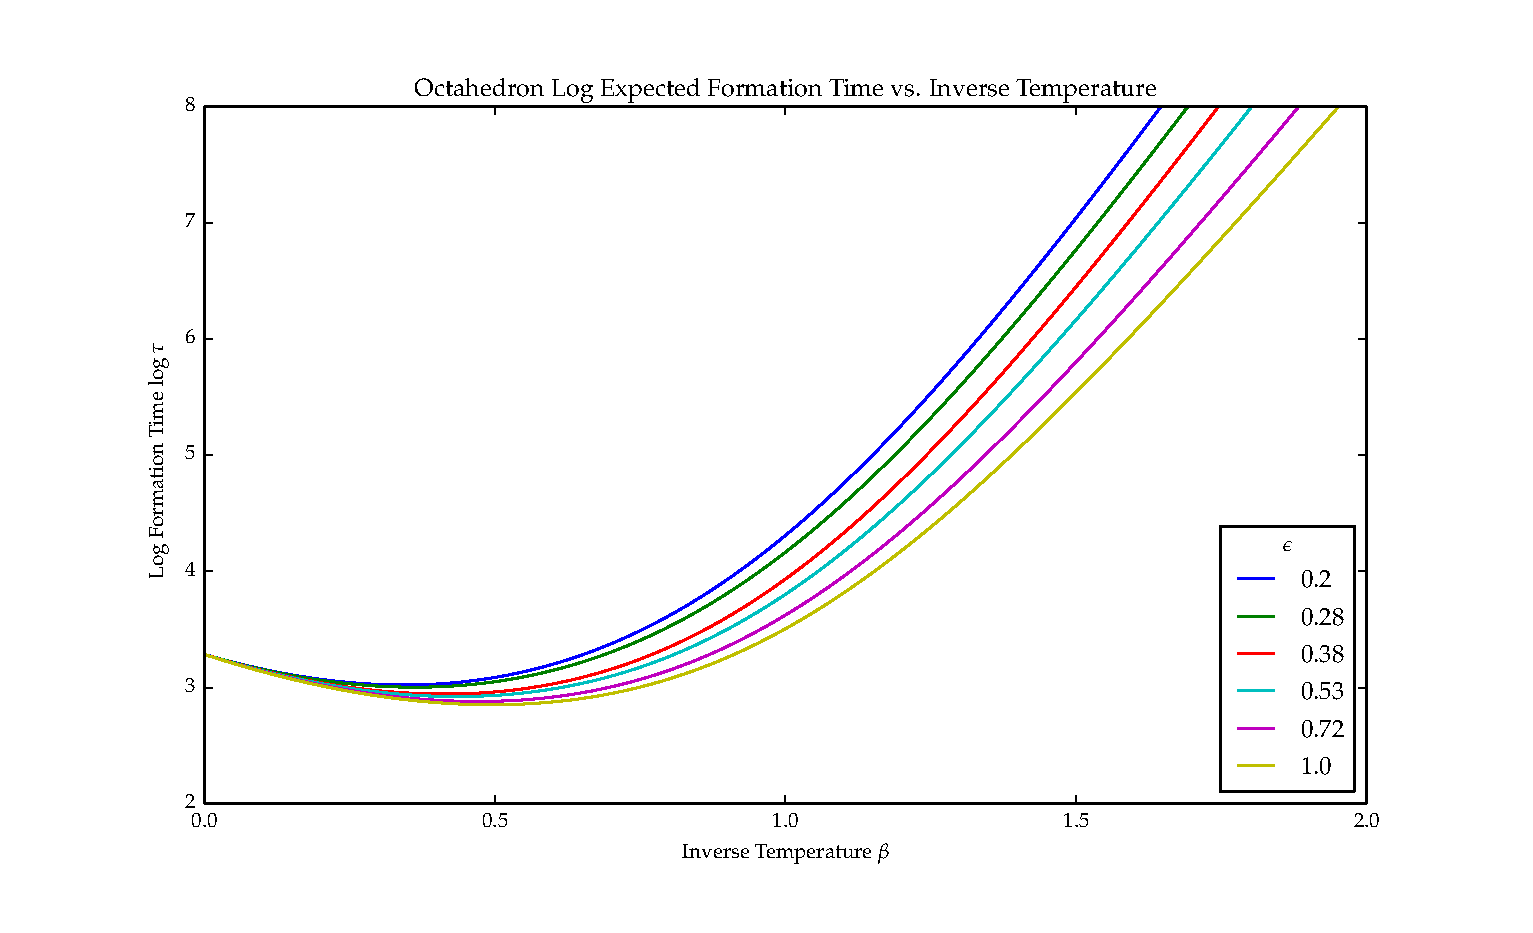
\includegraphics[scale=0.6]{images/octahedron_tau.eps}
\caption{Expected formation times for the octahedron as a function of $\epsilon$ and $\beta$.}
\end{figure}

